\documentclass[tikz,border=4pt]{standalone}
\usepackage[T1]{fontenc}
\usepackage{libertine}
\usepackage[scaled=0.92]{inconsolata}
\usepackage{xcolor}
\usepackage{tikz}
\usetikzlibrary{arrows.meta,positioning,calc}
\definecolor{stageblue}{HTML}{5B8FF9}
\definecolor{stagegreen}{HTML}{61DDAA}
\definecolor{stageorange}{HTML}{F6BD16}
\definecolor{stagered}{HTML}{E8684A}
\definecolor{linegray}{HTML}{667085}
\definecolor{softgray}{HTML}{F5F7FA}
\newcommand{\syscall}[1]{\texttt{#1}}
\begin{document}
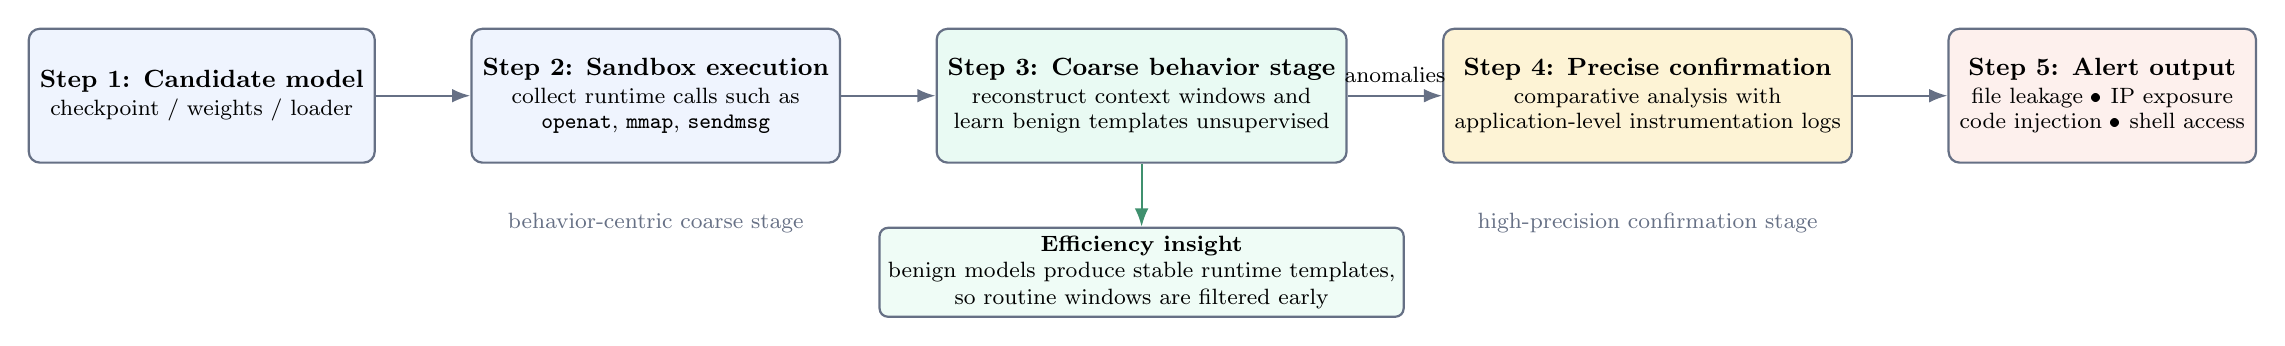
\begin{tikzpicture}[
  font=\small,
  >=Latex,
  line/.style={->, thick, draw=linegray},
  box/.style={rounded corners=4pt, draw=linegray, thick, minimum width=33mm, minimum height=17mm, inner sep=4pt, align=center},
  note/.style={rounded corners=3pt, draw=linegray, thick, inner sep=3pt, align=center, font=\footnotesize}
]

\node[box, fill=stageblue!10] (m) at (0,0) {\textbf{Step 1: Candidate model}\\[-1pt]\footnotesize checkpoint / weights / loader};
\node[box, fill=stageblue!10, right=12mm of m] (t) {\textbf{Step 2: Sandbox execution}\\[-1pt]\footnotesize collect runtime calls such as\\[-2pt]\footnotesize \syscall{openat}, \syscall{mmap}, \syscall{sendmsg}};
\node[box, fill=stagegreen!14, right=12mm of t] (u) {\textbf{Step 3: Coarse behavior stage}\\[-1pt]\footnotesize reconstruct context windows and\\[-2pt]\footnotesize learn benign templates unsupervised};
\node[box, fill=stageorange!18, right=12mm of u] (d) {\textbf{Step 4: Precise confirmation}\\[-1pt]\footnotesize comparative analysis with\\[-2pt]\footnotesize application-level instrumentation logs};
\node[box, fill=stagered!10, right=12mm of d, minimum width=37mm] (a) {\textbf{Step 5: Alert output}\\[-1pt]\footnotesize file leakage \textbullet{} IP exposure\\[-2pt]\footnotesize code injection \textbullet{} shell access};

\draw[line] (m) -- (t);
\draw[line] (t) -- (u);
\draw[line] (u) -- node[above=1pt, font=\footnotesize] {anomalies} (d);
\draw[line] (d) -- (a);

\node[note, fill=stagegreen!10, below=8mm of u, minimum width=40mm] (b) {\textbf{Efficiency insight}\\ benign models produce stable runtime templates,\\ so routine windows are filtered early};
\draw[->, thick, draw=stagegreen!65!black] (u.south) -- (b.north);

\node[font=\footnotesize, text=linegray, below=5mm of t] {behavior-centric coarse stage};
\node[font=\footnotesize, text=linegray, below=5mm of d] {high-precision confirmation stage};
\end{tikzpicture}
\end{document}
